\section{\CycForm s}
\label{s:DynAvers}
We begin with a brief review of main results of the periodic 
orbit theory, for a detailed introduction to the subject, we refer the reader to 
\refref{DasBuch}. Consider the evolution operator corresponding to an observable 
$a$ that is `additive' along every deterministic orbit $f^t(x)$:
\beq
	\Lop^t (y, x) = \delta (y - f^t (x)) e^{\beta A^t(x)} \, .
	\label{eq-EvOp}
\eeq
Here, $\beta$ is an auxilliary variable use of which will be apparent soon, 
$A^t (x)$ is the value of $a$ integrated along the orbit $f^t(x)$.
Since we required $a$ to be additive along the orbit and exponentiated
it in the definition of the evolution operator \refeq{eq-EvOp}, the
evolution operator itself is multiplicative:
\beq
	\Lop^{t_1 + t_2} (y,x) = \int dz \Lop^{t_2} (y, z) \Lop^{t_1} (z, x) \, . 
	\label{eq-SemiGroup}
\eeq
This semigroup property of the evolution operator allows us to define
the evolution operator as the formal exponential of its infinitesimal
generator \Aop :
\beq
	\Lop^t = e^{\Aop t} \, . 
	\label{eq-EvOpExp}
\eeq 
By definition \refeq{eq-EvOp}, eigenvalues and eigenfunctions of $\Lop^t$ (and 
thus \Aop ) are functions of $\beta$. Let us define $\rho_{\beta} (x)$ as the 
eigenfunction of \refeq{eq-EvOp} with the leading eigenvalue (the one with the 
largest real part); we can write the action of \refeq{eq-EvOp} on this density 
eplicitely as follows:
\beq
    \left[ \Lop^t \rho_{\beta} \right] (x) = e^{t s(\beta )} \rho_{\beta} (x) \, .
    \label{eq-EigenvalueRel}
\eeq
Here, $s(\beta)$ is the eigenvalue of $\Aop$. Note that for $\beta = 0$, 
\refeq{eq-EvOp} becomes the so called Perron-Frobenius operator (or transfer operator),
action of which simply evolves densities in time. If the system at hand is ergodic, 
$s(0) = 0$ and $\rho_0 (x)$ is called `invariant measure'. By evaluating the action 
of \refeq{eq-EvOp} for infinitesimal times one can show that long time average
(and higher moments) of the observable $a$ are given by the derivatives of $s(\beta)$:
\beq
    \langle a \rangle = \left. \frac{d s}{d \beta} \right|_{\beta = 0} \, , \quad
    \langle (a - \langle a \rangle )^2 \rangle = \left. \frac{d^2 s}{d \beta^2} 
                                                     \right|_{\beta = 0} \,, ...
    \label{eq-moments}                                                    
\eeq
In order to obtain $s(\beta)$ we construct the resolvent of \Aop , by taking the 
Laplace transform of \refeq{eq-EvOpExp}: 
\beq
	\int_0^{\infty} dt e^{-st} \Lop^t = (s-\Aop)^{-1} \, ,
	\label{eq-ResoolventA}
\eeq
trace of which peaks at the eigen values of \Aop. By taking the
Laplace transform of \refeq{eq-EvOp} and computing its trace 
by $\tr \Lop (y,x) = \int dx \Lop (x,x)$ we obtain the
classical trace formula:
\beq
\sum_{\alpha=0}^{\infty} \frac{1}{s-s_{\alpha}} = \sum_p T_p 
\sum_{r=1}^{\infty} \frac{e^{r(\beta A_p - s T_p)}}{\oneMinJ{r}} .
\ee{e-ClassicalTraceFormula}
which relates the spectrum of \Aop\ to the spectrum of the periodic 
orbits. Here, $s_{\alpha}$ are the eigenvalues of \Aop , 
outer sum on the RHS runs over the `prime cycles' of the system, 
$T_p$ is the period of the prime cycle $p$, $A_p$ is the value of 
the observable along the prime cycle, $s$ is the auxilliary
variable of the Laplace transform, and $\monodromy_p$ is the transverse 
monodromy matrix, eigenvalues of which are the Floquet multipliers of the prime 
cycle $p$ excluding the marginal ones ($|\Lambda| \neq 1$). In deriving  
\refeq{e-ClassicalTraceFormula} one assumes a single marginal direction, namely 
the direction that is parallel to the periodic orbit at all times, and evaluates 
the trace integral by transforming to a local coordinate system where one of the 
coordinates is paralel to the flow while the rest is transverse. Integration along
the parallel direction contributes factors of $T_p$, and the transverse integral
over the delta function contributes $\oneMinJ{r}$. Important observation is that
the final result \refeq{e-ClassicalTraceFormula} do not depend on the choice
of the coordinate system. In the \twomode\ system, we have an extra unit Floquet
multiplier for the symmetry direction, however, if we assume that we are working
in the \slice , and define all of our observables within the \slice , we can 
simply ignore this direction and apply \refeq{e-ClassicalTraceFormula} and what
follows using non-marginal Floquet multipliers. 

While the classical trace formula \refeq{e-ClassicalTraceFormula} manifests 
the essential duality between the spectrum of an observable and that of 
the periodic orbits, in practice, it is hard to work with since the eigenvalues 
are located at the poles of \refeq{e-ClassicalTraceFormula}. For this reason, 
one expresses this duality equivalently as the following spectral determinant
\beq
    \det (s-\mathcal{A}) = \exp \left( - \sum_p \sum_{r=1}^{\infty}
                             \frac{1}{r} \frac{e^{r(\beta A_p - s T_p)}}{\oneMinJ{r}} \right)\, ,
\ee{e-SpectralDeterminant}
logarithmic derivative of which gives \refeq{e-ClassicalTraceFormula}. 
The spectral determinant \refeq{e-SpectralDeterminant} is easier to work 
with since the spectrum of $\mathcal{A}$, is now located at the zeros of 
\refeq{e-SpectralDeterminant}. Convergence of \refeq{e-SpectralDeterminant} 
is still not obvious. More insight is gained by approximating $\oneMinJ{r}$ 
by the product of expanding Floquet multipliers and then computing the $r$ 
sum in \refeq{e-SpectralDeterminant}.
\bea
\oneMinJ{} &=& | (1 - \ExpaEig_{e,1})(1 - \ExpaEig_{e,2})... \continue
			&&(1 - \ExpaEig_{c,1}) (1 - \ExpaEig_{c,2}) ... | \nonumber \\
			&\approx& \prod_e |\ExpaEig_e| = |\ExpaEig_p|,
\eea
where $|\ExpaEig_{e,i}| > 1$ and $|\ExpaEig_{c,i}| < 1$ are expanding and contracting Floquet multipliers respectively. After this approximation, $r$-sum in \refeq{e-SpectralDeterminant} becomes the Taylor expansion of natural logarithm and it can be compactly written as follows:
\beq
1 / \zeta = \prod_r (1 - t_p) \, \mbox{where}, \, t_p = \frac{1}{|\ExpaEig_p|} e^{\beta A_p - s T_p} z^{n_p} .
\ee{e-DynamicalZeta}
Where we inserted the `order tracking' term $z$. For complete binary symbolic dynamics, the dynamical zeta function \refeq{e-DynamicalZeta} can be brought into the `curvature expansion' form:
\bea
1 / \zeta &=& 1 - t_0 - t_1 - (t_{01} - t_0 t_1 )  \label{e-CycleExpansion} \\
		  && - [(t_{011} - t_{01}t_1) + (t_{001} - t_{01} t_0)] - ... \continue
		  &=& 1 - \sum_f t_f - \sum_n \hat{c}_n \label{e-CurvatureExpansion}.
\eea
In the curvature expansion \refeq{e-CurvatureExpansion}, we grouped the 
contributions to the dynamical zeta function as `fundamental' contributions 
$t_f$ and `curvature' corrections. One expects the curvature corrections to 
be small since the longer prime cycles are `shadowed' by the combination of 
the shorter ones, the `pseudocycles'.

For complete binary symbolic dynamics, the only fundamental contributions to 
the dynamical zeta function are the cycles with topological length $1$, see 
\refeq{e-CurvatureExpansion}. This is not the case for any map since in general 
there might be non-trivial pruning rules, hence longer cycles can appear unshadowed. 
The Poincar\'e return map of \reffig{fig:psectandretmap}\,{d) is such a map 
with non-trivial pruning rules, however, note that cycles \cycle{001} and \cycle{011} 
passes very close to the tip of the cusp, the critical point, in 
\reffig{fig:psectandretmap}\,{d). This observation motivates us to approximate 
the return map of \reffig{fig:psectandretmap}\,{d), as if its tip is located at 
$s = 0.97986453$, where the cycle \cycle{001} lands, and omit the contributions 
above this point. We will refer this approximation as the `finite grammar approximation' 
since by doing it, we obtain single pruning rule; that is the symbol sequence 
$00$ is not allowed. This grammar is known as the `golden mean' pruning and a 
complete binary symbolic dynamics can be converted to the golden mean symbolic 
dynamics by substitution $0 \rightarrow 01$. We can write the dynamical zeta 
function for the golden mean pruned symbolic dynamics by replacing $0$s in 
\refeq{e-CycleExpansion} by $01$:
\bea
1 / \zeta &=& 1 - t_{01} - t_1 - (t_{011} - t_{01} t_1 ) \label{e-GoldenMeanCycleExpansion}\\
		  && - [(t_{0111} - t_{011}t_1) + (t_{01011} - t_{01} t_{011} ) ] - ... \nonumber
\eea
Note that all the contributions longer than topological length $2$ to the golden mean dynamical zeta function are in form of shadowing combinations. However, as we shall see, they are not small.

While dynamical zeta functions are useful for investigating the convergence 
properties, they are not exact, and their computational cost is same with 
that of the exact spectral determinants. For this reason, we will expand the 
spectral determinant \refeq{e-SpectralDeterminant} ordered in the topological 
length of cycles and pseudocycles as follows:
\beq
    \det (s-\mathcal{A}) =   \prod_p \exp \left( - \sum_{r=1}^{n_p r < N}
                             \frac{1}{r} \frac{e^{r(\beta A_p - s T_p)}
                                          }{\oneMinJ{r}} z^{n_p r} \right) \, .
\ee{e-SpectralDeterminantExp}
This is the form that we use to compute the spectral determinant. For each prime 
cycle, we compute the sum term in \refeq{e-SpectralDeterminantExp} truncated at 
the expansion order $N$, and then expand the exponential upto order $N$, and multiply 
this expansion with the contributions from previous cycles and drop terms with 
order greater than $N$. This way, we obtain the $N^{th}$ order spectral determinant 
\refeq{e-SpectralDeterminant}. Let us denote the resultant series after setting $z=1$ as
\beq
    F_N(s, \beta ) = 1 - \sum_{n=1}^{N} Q_n(s, \beta ) \, .
    \label{e-NthOrderSpectDet}
\eeq
Remember that we are searching for the eigenvalues $s ( \beta)$ of the \Aop , more
specifically, we would like to compute the moments \refeq{eq-moments}. $s ( \beta)$
are located at the zeros of the spectral determinant, hence they satisfy the implicit
equation:
\beq
    F_N(s, s(\beta )) = 0 \, .
    \label{e-FNimplicit}
\eeq
By taking derivative of \refeq{e-FNimplicit} with respect to $\beta$ and applying
chain rule we obtain
\beq
    \frac{d s}{d \beta} = - \left. \frac{\partial F}{\partial \beta} \right/
                                     \frac{\partial F}{\partial s}
\eeq
We can similarly take the higher order derivatives to get higher order moments. 
Finally, by defining 
\beq
	\langle T \rangle_N = \left. \partial F_N / \partial s \right|_{\beta=0, s=s (0)}
	\label{eq-Tavg}
\eeq
we obtain the \CycForm s:
\bea
    \langle a \rangle_N &=& - \frac{1}{\langle T \rangle_N} \left.
                              \frac{\partial F_N}{\partial \beta}
                              \right|_{\beta=0, s=s (0)} \, ,   \label{e-Avga} \\
    \langle (a - \langle a \rangle )^2 \rangle_N
    &=& - \frac{1}{\langle T \rangle_N} \left. \frac{\partial^2 F_N}{\partial \beta^2} \right|_{\beta=0,
                                                                    s=s (0)} \, \label{e-Avgsigma} .
\eea
While for an invariant measure we expect $s (0)$ to be $0$, we did not make such
substitution in \CycForm s, since in practice, our approximation to the spectral
determinant is always of a finite precision, hence the solution of 
$F_N(0, s(0)) = 0$ is not exactly $0$. This eigenvalue has a special meaning:
since it is the leading eigenvalue of the Perron-Frobenius operator, it determines
how much the dominant measure decays in time (see \refeq{eq-EigenvalueRel} ). With
this interpretation, we define $\gamma = - s(0)$ as the `escape rate'. This quantity
has a certain meaning in our finite grammar approximation; it tells us how frequently
does the flow visit the part of the attractor that we cut off within the approximation.

We defined $\langle T \rangle$ in \refeq{eq-Tavg} as a shorthand for a partial
derivative, however, we can also develop and interpretation for it by looking at
definitions of dynamical zeta function \refeq{e-DynamicalZeta} and the spectral 
determinant \refeq{e-SpectralDeterminant}. In both series, partial derivative with
respect to $s$ turns them into weighted sum of the cycle periods; with this intuition, 
we define $\langle T \rangle$ as the `mean cycle period'.

We constructed the spectral determinant \refeq{e-NthOrderSpectDet} at different 
orders for two observables: phase velocity $\dot{\phi}$ and the leading Lyapunov 
exponent. Note that $A_p$ appearing in \refeq{e-SpectralDeterminantExp} is the
integrated observable, so in order to obtain the moments of phase velocity and
Lyapunov exponent from \refeq{e-Avga} and \refeq{e-Avgsigma}, we respectively input 
$A_p = \phi_p$ phase shift of the prime cycle, and $A_p = \ln |\Lambda_p|$ logarithm
of the expanding Floquet multiplier of the prime cycle. 

In \refsect{s:visual}, we explained that \SOn{2} phase shifts corresponds to 
the drifts in the configuration space, with this in mind, we can relate the 
variance of phase velocity to the diffusion constant of our system:
\beq
    D = \frac{1}{2 d} \sigma_{\dot{\phi}}^2 
      = \frac{\langle (\dot{\phi} - \langle \dot{\phi} \rangle)^2 \rangle}{2} ,
\eeq
where $d=1$ since our configuration space is one dimensional. 

\reftab{t-DynamicalAverages} and \reftab{t-DynamicalAveragesNoGrammar} shows
the cycle averages of the escape rate ($\gamma$), mean period ($\langle T \rangle$),
leading Lyapunov exponent ($\Lyap$), mean phase velocity ($\langle \dot{\phi} \rangle$)
and the diffusion constant ($D$) respectively within and without the finite grammar 
approximation. In the latter, we input all the \rpo s we have found into the expansion
\refeq{e-SpectralDeterminantExp}, whereas in the former, we discarded the cycles
with symbol sequence `00'.

\begin{table}
	\begin{tabular}{c|c|c|c|c|c}
	 $N$ & $\gamma$ & $\langle T \rangle$ & $\lambda$ & $\langle \dot{\phi} \rangle$ & $D$ \\ 
	\hline
	1 & 0.24983007 & 3.64151210 & 0.10834935 & 0.02223518 & 0.00090019 \\ 
 	2 & -0.01159743 & 5.89675999 & 0.10302904 & -0.14242535 & 0.22615040 \\ 
 	3 & 0.02744646 & 4.72713874 & 0.11849781 & -0.14916163 & 0.22541882 \\ 
 	4 & -0.00445545 & 6.23866097 & 0.10631075 & -0.22271184 & 0.54199883 \\ 
 	5 & 0.00068106 & 5.89674866 & 0.11842709 & -0.19506985 & 0.47091930 \\ 
 	6 & 0.00068491 & 5.89688492 & 0.11820055 & -0.21660997 & 0.64918118 \\ 
 	7 & 0.00063044 & 5.90316812 & 0.11835165 & -0.18083296 & 0.51935080 \\ 
 	8 & 0.00071488 & 5.89189180 & 0.11827587 & -0.21129228 & 0.78673581 \\ 
 	9 & 0.00072867 & 5.88975993 & 0.11826879 & -0.19203222 & 0.70977900 \\ 
 	10 & 0.00072808 & 5.88986409 & 0.11826793 & -0.20302879 & 0.90493496 \\ 
 	11 & 0.00072790 & 5.88989901 & 0.11826783 & -0.19453187 & 0.86683629 \\ 
 	\end{tabular}
	\caption{Cyle expansion estimates of the escape rate $\gamma$, average cycle period $\langle T \rangle$, Lyapunov exponent $\lambda$, average phase velocity $\langle \dot{\phi} \rangle$ and the diffusion coefficient $D$ with respect to the expansion order $N$ .}
	\label{t-DynamicalAverages}
\end{table}
\begin{table}
	\begin{tabular}{c|c|c|c|c|c}
	 $N$ & $\gamma$ & $\langle T \rangle$ & $\lambda$ & $\langle \dot{\phi} \rangle$ & $D$ \\ 
	\hline
	1 & 0.24982996 & 3.64151221 & 0.10834917 & 0.02223518 & 0.00090019 \\ 
 	2 & -0.01159761 & 5.89676053 & 0.10302891 & -0.14242516 & 0.22615014 \\ 
 	3 & 0.02261469 & 4.88995874 & 0.13055574 & -0.16698925 & 0.28645997 \\ 
 	4 & -0.00606560 & 6.24822611 & 0.11086469 & -0.22623282 & 0.55402655 \\ 
 	5 & 0.00091264 & 5.77716415 & 0.11812034 & -0.19839015 & 0.47840111 \\ 
 	6 & 0.00026210 & 5.83645342 & 0.11948918 & -0.21788301 & 0.65393430 \\ 
 	7 & 0.00001771 & 5.86382098 & 0.12058951 & -0.18565119 & 0.55022944 \\ 
 	8 & 0.00011328 & 5.85110445 & 0.12028459 & -0.21480977 & 0.80768111 \\ 
 	9 & 0.00017071 & 5.84222727 & 0.12010579 & -0.19376222 & 0.72685211 \\ 
 	10 & 0.00015683 & 5.84466944 & 0.12014022 & -0.20501316 & 0.92174228 \\ 
 	\end{tabular}
	\caption{Cyle expansion estimates of the escape rate $\gamma$, average cycle period $\langle T \rangle$, Lyapunov exponent $\lambda$, average phase velocity $\langle \dot{\phi} \rangle$ and the diffusion coefficient $D$ with respect to the expansion order $N$ .}
	\label{t-DynamicalAveragesNoGrammar}
\end{table}


\begin{figure}%[H]
\centering
 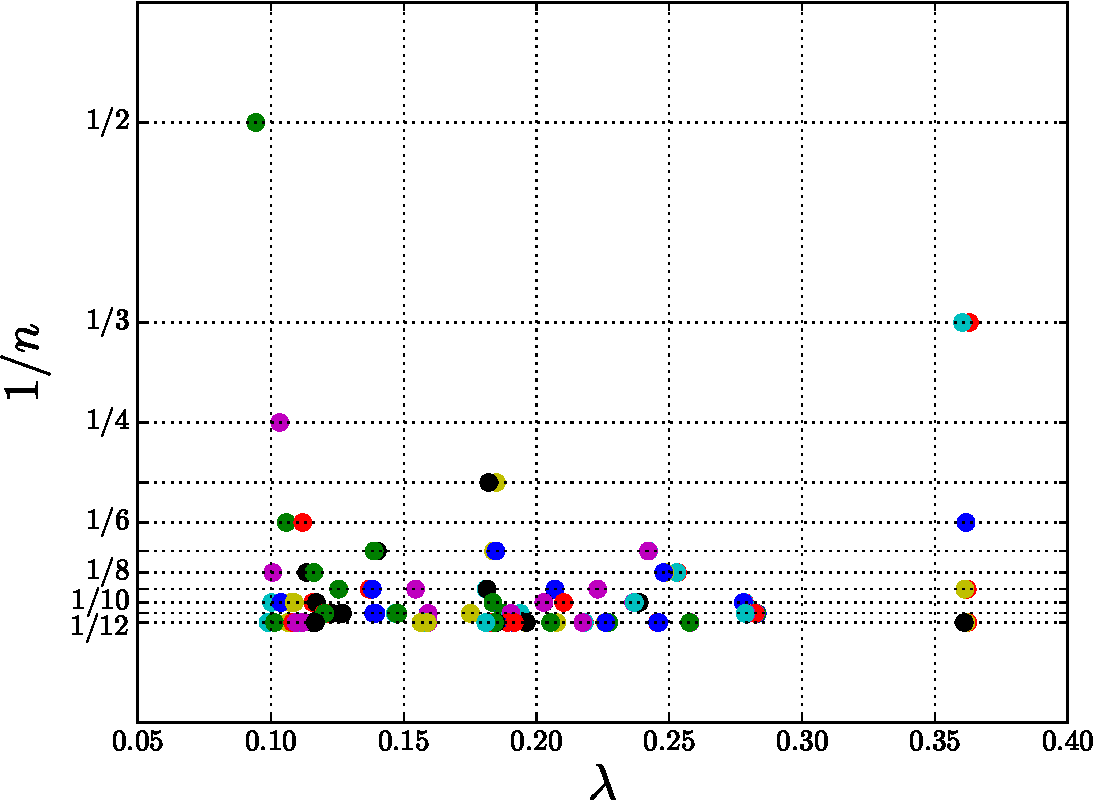
\includegraphics[width=0.45\textwidth]{2modes-lambdaDist}
\caption{Distribution of the leading Floquet exponents of \twomode\ cycles.}
\label{f-2modes-lambdaDist}
\end{figure}

We motivated our finite grammar approximation by expecting a fast convergence 
due to the nearly exact shadowing combinations and we can clearly see this 
by comparing numbers in 
\reftab{t-DynamicalAverages} and \reftab{t-DynamicalAveragesNoGrammar}.
Take, for example, Lyapunov exponent which converges with $7$ digit accuracy
at the final order in \reftab{t-DynamicalAverages} while we have only $4$ digits 
at this order in \reftab{t-DynamicalAveragesNoGrammar}. Other observables compares
similarly in terms of their convergence in both cases. Note, however, that the 
escape rate in \reftab{t-DynamicalAverages} converges to $\gamma = 0.000727889$,
whereas in \reftab{t-DynamicalAveragesNoGrammar} it gets smaller and smaller
with an oscillatory behavior. This is due to the fact that in the finite grammar
approximation, we neglect a definite piece of attractor that corresponds to the 
cusp of the return map in \reffig{fig:psectandretmap} (d), above the part that 
is cut by \cycle{001}.

In order to compare with the cycle averages, we numerically estimated the
leading Lyapunov exponent of the \twomode\ system using the method of
Wolf \etal\rf{WolfSwift85}. This procedure was repeated 100 times for
different initial conditions, yielding a mean estimate of
$\Lyap_{Numerical} = 0.1198 \pm 0.0008$. While the finite grammar
estimate $\Lyap_{FG} = 0.1183$ is within $0.6\%$ range of this value,
the full cycle expansion agrees with the numerical estimate. This is not
surprising, since in the finite grammar approximation, we discard the
most unstable cycles, thus, we obtain a slightly smaller Lyapunov
exponent while obtaining a better convergence.
